
%(BEGIN_QUESTION)
% Copyright 2009, Tony R. Kuphaldt, released under the Creative Commons Attribution License (v 1.0)
% This means you may do almost anything with this work of mine, so long as you give me proper credit

Two temperature switches sense the temperature inside an electrically-heated oven, each one with its own ``trip'' value.  Examine the schematic diagram for the control circuit, and then explain how it is supposed to function:

$$\includegraphics[width=15.5cm]{i04005x01.eps}$$

Suppose relay contact CR1 were to fail open.  Identify the effect this fault would have on the operation of the temperature control circuit.

\vskip 20pt \vbox{\hrule \hbox{\strut \vrule{} {\bf Suggestions for Socratic discussion} \vrule} \hrule}

\begin{itemize}
\item{} This type of control system is sometimes called {\it differential gap}.  Explain why this label is appropriate for describing the system's operation.
\item{} Sketch a modified version of this circuit whereby the same temperature switches and relay control power to a three-phase electric heating element powered by 480 VAC.
\item{} Explain the effect(s) of the vertical wire connecting between the two temperature switches were to fail open.
\item{} Explain the effect(s) of the 285 $^{o}$F temperature switch failing open.
\item{} Explain the effect(s) of the 285 $^{o}$F temperature switch failing shorted.
\item{} Explain the effect(s) of the 250 $^{o}$F temperature switch failing open.
\item{} Explain the effect(s) of the 250 $^{o}$F temperature switch failing shorted.
\end{itemize}

\underbar{file i04005}
%(END_QUESTION)





%(BEGIN_ANSWER)

The temperature should cycle between 250 and 285 degrees F, with the relay ``latching'' the heating element on even after the lower-temp switch contacts open.  This is sometimes called a {\it differential gap} control system because the process variable bounces back and forth within a ``gap'' established by two setpoint values.

\vskip 10pt

If contact CR1 fails open, the relay cannot latch.  Thus, the heater will turn off any time the lower-temperature switch trips.  The result of this will be a much more rapid cycling, with the temperature centered somewhere around 250 degrees.

%(END_ANSWER)





%(BEGIN_NOTES)


\vskip 20pt \vbox{\hrule \hbox{\strut \vrule{} {\bf Virtual Troubleshooting} \vrule} \hrule}

This question is a good candidate for a ``Virtual Troubleshooting'' exercise.  Presenting the diagram to students, you first imagine in your own mind a particular fault in the system.  Then, you present one or more symptoms of that fault (something noticeable by an operator or other user of the system).  Students then propose various diagnostic tests to perform on this system to identify the nature and location of the fault, as though they were technicians trying to troubleshoot the problem.  Your job is to tell them what the result(s) would be for each of the proposed diagnostic tests, documenting those results where all the students can see.

During and after the exercise, it is good to ask students follow-up questions such as:

\begin{itemize}
\item{} What does the result of the last diagnostic test tell you about the fault?
\item{} Suppose the results of the last diagnostic test were different.  What then would that result tell you about the fault?
\item{} Is the last diagnostic test the best one we could do?
\item{} What would be the ideal order of tests, to diagnose the problem in as few steps as possible?
\end{itemize}

%INDEX% Measurement, temperature: switch

%(END_NOTES)


